\chapter{相关研究进展}
\section{引言}
自从计算机技术应用到医学影像分析以来,有许许多多医学影像分析难题因其具有的重大临床应用价值和实际意义而引起研究者的浓厚兴趣并为之投入大量时间和精力,生物标记物的精确定位便是其中之一。本章将会生物标记物精确定位任务的常用数据集进行介绍。接着将会介绍本文方法中涉及到的最为重要的基本知识点,包括卷积神经网络、对抗生成网络和自编码-解码器。
下一步,我们将对可用于完成生物标记物精确定位任务的方法进行详细(包括传统的多示例学习和当下流行的卷积神经网络方法)介绍,力求将相关方法阐述得清晰明了,突出比较各种方法在生物标记物的精确定位任务上的长处和不足。在本章最后,我们将给出实验结果的评判标准,并阐述选择这些比较标准的合理性。

\section{常用数据集}
一旦展开对选取问题的具体研究,第一步便是选取实验所使用的数据集。尤其对于当下十分火热、有着数据驱动特性的卷积神经网络来说,选择一个合适的数据集的重要性更加不言而喻。再加上医学影像数据获取、标注成本更高,导致可用于生物标记物的精确定位测试的公开数据集较少。由于医学数据很可能会涉及到病人的隐私,为了尽可能保护病人权益,防止病人信息泄露,图像数量较多的、图像质量较高的数据集往往存于知名公立医院且未公开。在已然公开的数据集中,本文将选取一些知名度较高的、在学术界被研究者广泛接受的、图像质量相对较高的数据集进行介绍。

\subsection{眼底病变数据集}
眼科学是临床医学的一个独特分支。眼科的影像学检查方法有眼底摄影、光学相干断层扫描、眼底荧光血管造影、扫描激光检眼镜等。一个明确的眼科疾病诊断需要结合几个不同的试验结果。在临床实践中,诊断和治疗策略的确定依赖于影像学资料的评价。目前眼底照片已广泛应用于青光眼和视网膜疾病等眼科疾病的诊断。然而,眼成像数据的解释需要大量的经验和时间。在这里,我们介绍部分具有良好注释和标签的数据集,扼要信息如表~\ref{tab:datasets_info}所示,下面分别进行简单介绍。

注意,图像级标注指的是将图像标注为对应类别,如正常/异常。像素级标注在图像级标注基础上还标出病变的准确位置。另外,图像数量指的是数据集中官方有提供标注的图像数据。以上说明同样适用于表~\ref{tab:skin_datasets_info}。

\begin{table}[h]
	\centering
	\caption{常用眼底病变数据集。}		
	\label{tab:datasets_info}
	\begin{tabular}{c|c|c|c}
		\toprule[2pt]
		数据集名称 & 图像数量 & 类别 & 标注 \\
		\midrule[2pt]
		Kaggle Diabetic Retinopathy (DR)	& 35,127	& 5	&图像级 \\
		\hline                         
		iChallenge Glaucomatous Optic Neuropathy (GON)    & 1,200    & 2 & 图像级 \\ \hline
		iChallenge Age-related Macular Degeneration (AMD) & 1,200    & 2 & 部分像素级 \\ \hline
		iChallenge Pathological Myopia (PM)               & 1,200    & 2 & 部分像素级 \\ \hline
		ODIR-5K & 7,000 & 8 & 图像级 \\ \hline
		
		Indian Diabetic Retinopathy Image Dataset (IDRiD) & 516 & 5 & 部分像素级 \\
		\bottomrule[2pt]
	\end{tabular}
\end{table}

糖尿病视网膜病变是发达国家劳动年龄人口失明的主要原因。DR数据集\footnote{https://www.kaggle.com/c/diabetic-retinopathy-detection/data}是目前关于糖尿病视网膜病变的最大数据集,提供了在各种成像条件下拍摄的高分辨率视网膜图像。目前在Kaggle上开源数据中,训练集有35,127张样本,每张图像尺寸均大于$1000\times 1000$但大小不等,目前只有图像集标注。专业医师根据患者患病程度将每张图像标注为0至4共5类。0、1、2、3和4分别代表未患糖尿病视网膜病变、轻微糖尿病视网膜病变、中度糖尿病视网膜病变、严重糖尿病视网膜病变和增生性糖尿病视网膜病变。标注数字越大代表患病越严重。

GON数据集\footnote{http://ai.baidu.com/broad/subordinate?dataset=gno}是关于青光眼眼底照片的数据集,共包含1,200张彩色眼底照片。并平均分为训练集、验证集和测试集。其中,训练集图像由德国蔡司眼底照相机拍摄,尺寸大小为$2124\times 2056$,验证集和测试集图像由佳能眼底照相机拍摄,尺寸大小为$1634\times 1634 $。所有图像均是图像集标注,标记为青光眼/非青光眼,均以后极为中心,伴有黄斑和视盘。

AMD数据集\footnote{http://ai.baidu.com/broad/subordinate?dataset=amd}是关于年龄相关性黄斑变性眼底照片数据库,共有1,200张彩色眼底照片可供选择。这些照片来自非AMD受试者(约77\%)和AMD患者(约23\%)。提供AMD/非AMD的标签,椎间盘边界和中央凹的位置,以及各种病变的边界,以训练模型进行自动AMD评估。数据集中每个样本都有图像级标注,只有部分样本有像素级标注,标注了与年龄相关性黄斑变性相关的四种典型异常。

近视已成为全球公共卫生的负担。为了促进近视的研究,PM数据集\footnote{http://ai.baidu.com/broad/subordinate?dataset=pm}是病理性近视眼底照片数据库,提供了1200个来自非病理性近视受试者和病理性近视患者(约50\%)的标注视网膜眼底图像的大数据集。每个图像样本同样均有图像级标注,部分图像有包括斑片状视网膜萎缩(包括乳头周围萎缩)和视网膜脱离在内的两种典型异常的像素级标注。

ODIR-5K数据集\footnote{https://odir2019.grand-challenge.org/dataset/}是一个结构化的眼科数据库,其中包括5,000名患有年龄的患者,双眼的彩色眼底照片和医生的诊断关键词。注意只有3,500名患者(7,000张样本)数据作为训练集,并且有图像级标签。该数据集是上工医疗技术有限公司从中国不同医院/医疗中心收集的“真实”患者信息。专业医师将患者分为8个标签,包括正常,糖尿病,青光眼,白内障,年龄相关性黄斑变性,高血压,近视和其他疾病/异常。由于存在部分病人同时患有多种疾病,因而部分图像有多个标签。

IDRiD\footnote{https://idrid.grand-challenge.org/Data/}眼底图像是由印度一家眼科诊所的视网膜专家收集的。数据集共包括516张样本,均提供了典型糖尿病视网膜病变病变和正常视网膜结构的专家标记。数据集所有图像都集中在黄斑附近。图像分辨率为$4288\times 2848$像素,存储为jpg文件格式。此外,它还根据国际临床相关性标准,为数据库中的每张图像提供关于糖尿病视网膜病变的疾病严重程度和糖尿病黄斑水肿的信息。与DR数据集一样,它一共将图像分为5类。与DR数据集不同的是,IDRiD数据集有81张患病彩色眼袋图像有精确像素级标注,如微动脉瘤、软渗出物、硬渗出物和出血。

眼底病变往往有病变区域较小,病变区域数量较多,病变区域分布较分散的特点。因此,眼底有些病变区域容易混淆,比较难发现。另外,眼底图像较为精细,各种细节纹理丰富,故发现眼底病变的生物标记物通常极具挑战性。

\subsection{黑色素瘤皮肤病变图像}
黑色素瘤是多种皮肤癌中最致命的一种。黑色素瘤是发生在皮肤表面的色素性病变,可以通过专业医师的视觉检查早期发现。黑色素瘤也适用于自动检测与图像分析。皮肤镜检查是一种皮肤成像方法,与无辅助的视觉检查相比,已证明可改善皮肤癌的诊断。为了更广泛地提供专业知识,国际皮肤成像协作组织开发了专门档案,这是一个国际皮肤镜图像库,可用于皮肤科专业医师的临床培训,也能用于举办比赛,寻求计算机算法解决临床问题。在这里,我们介绍三个图像质量较高,可用于生物标记物定位的黑色素瘤病变数据集。数据集名称、图像数量等基本信息如表~\ref{tab:skin_datasets_info}所示。


\begin{table}[h]
	\centering
	\caption{常用眼底病变数据集。}		
	\label{tab:skin_datasets_info}
	\begin{tabular}{c|c|c|c}
		\toprule[2pt]
		数据集名称 & 图像数量 & 类别 & 标注 \\
		\midrule[2pt]
		
		International Skin Imaging Collaboration (ISIC) 2017 &  $\sim 2,300$ & 3 & 部分像素级 \\ \hline
		International Skin Imaging Collaboration (ISIC) 2018 & $\geq 12,500$ & 7  & 部分像素级 \\ \hline
		International Skin Imaging Collaboration (ISIC) 2019 & 25,331 & 8  & 图像级  \\ 
		\bottomrule[2pt]
	\end{tabular}
\end{table}

ISIC2017数据集~\cite{codella2018skin}中大约有2,300张皮肤镜图像,其中大约2,150张图像是训练集,剩下约150张图像是验证集。图像尺寸大小在$400\sim 600$之间。数据集包括黑色素瘤、脂溢性角化病和良性的痣(可看做正常)在内的3种类别。

ISIC2018数据集~\cite{codella2019skin, tschandl2018ham10000}中有超过12,500张皮肤镜图像。图像尺寸大小在$400\sim 600$之间。包括光化性角化病(日光性角化病)和上皮内癌(鲍文氏病)、基底细胞癌、良性的角化病、皮肤纤维瘤、黑素细胞痣、黑素瘤、血管皮肤损伤共7类。

ISIC2019数据集\footnote{https://challenge2019.isic-archive.com/}中有25,331张皮肤镜图像,包括黑色素瘤黑素细胞痣、基底细胞癌、光化性角化病、良性角化病(太阳扁豆/脂溢性角化病/扁平苔藓样角化病)、皮肤纤维瘤、血管病变、鳞状细胞癌和没有以上病变类型在内的8个类别。图像尺寸大小在$400\sim 600$之间。

与眼底病变类型不同的是,黑色素瘤的各种病变类型往往在皮肤镜上所占区域比较大,通常所占比例在$1/3$以上。各种病变类型之间的区别主要表现在病变区域细微纹理区间上。

\section{基本知识要点}
本小节主要是介绍生物标记物定位任务的概念和目前常用的模型方法。首先,我们会介绍生物标记物的概念,让读者对本文研究主题有清晰的认识。接着会介绍卷积神经网络、自动编码器-解码器等重要基本要点。下一步介绍目前已有的常用解决模型方法。最后介绍对各种模型方法性能比较的评价标准。
\subsection{卷积神经网络}
\begin{figure}[h]
	\centering
	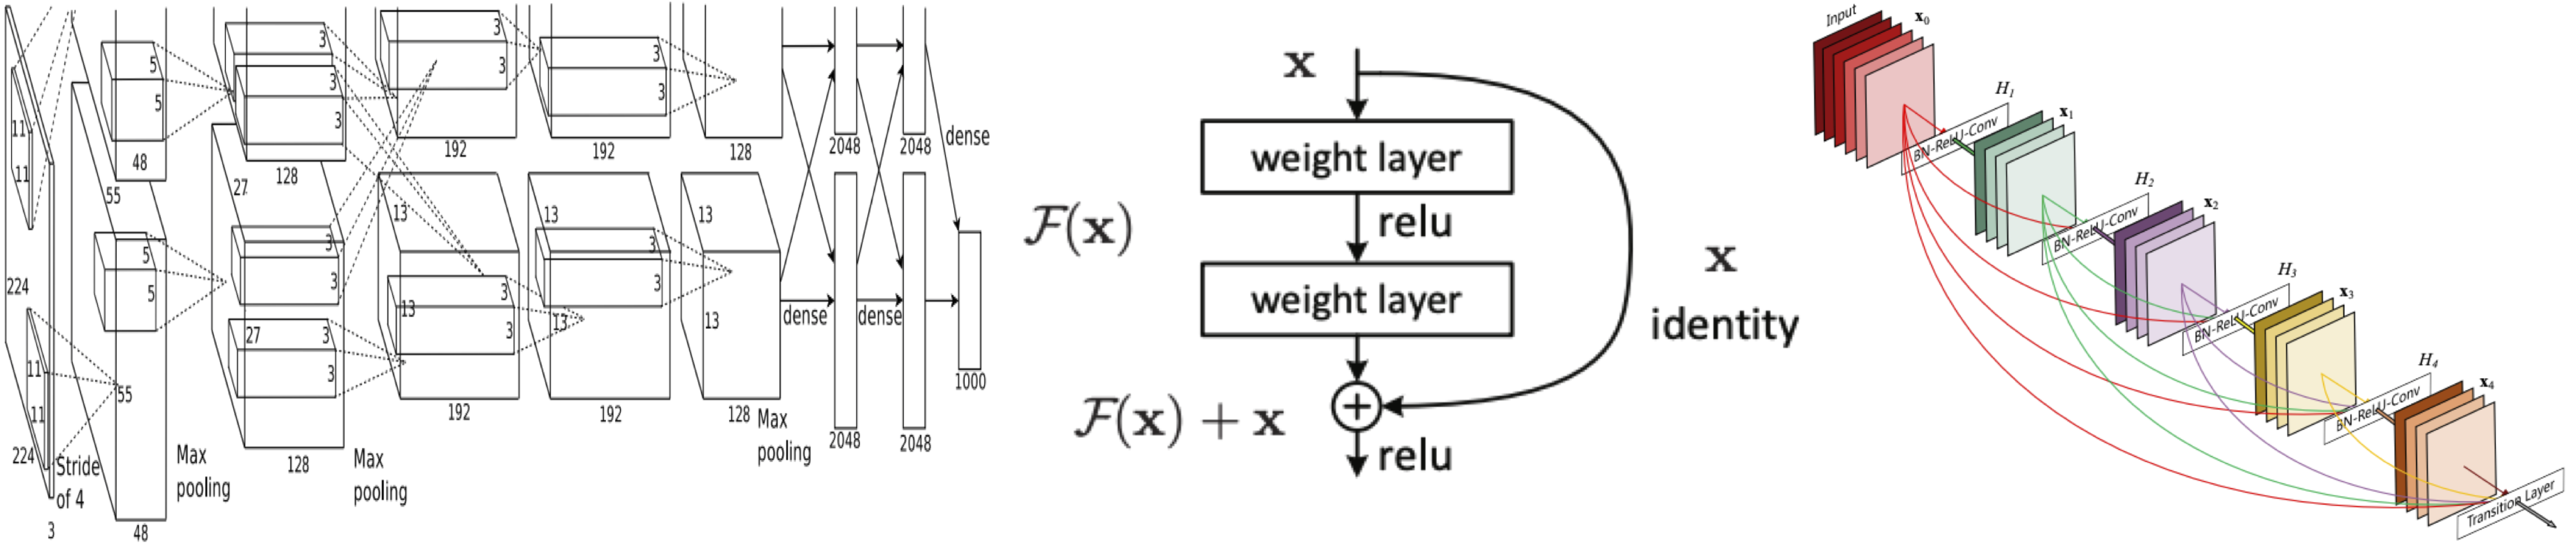
\includegraphics[width=1.0\textwidth]{figure/popular_networks}
	\caption{三种经典的卷积神经网络模型结构。从左到右,依次为AlexNet~\cite{krizhevsky2012imagenet}、ResNet~\cite{he2016deep, he2016identity}、DenseNet~\cite{huang2017densely}(图片均来自于原始论文)。注意,中间是ResNet的一个残差单元,ResNet实际上是由多个残差单元堆叠组成。} 
	\label{fig:popular_networks}
\end{figure}
卷积神经网络最初是为了避免传统神经网络(多层感知机~\cite{gardner1998artificial})在处理图像时的缺点而提出的。多层感知机在处理图像数据时,多层感知机对每张输入图像中的每个像素点都使用一个感知器。对于较大的图像,权重的数量很快就变得难以管理。例如,对于一个有3个彩色通道的224$\times$224像素图像,大约需要训练150,000个权值。此时,多层感知机的训练将变得十分困难。另外,多层感知机不具备平移不变性。例如,如果一张猫出现在一张图像的左上角和另一张图像的右下角,多层感知机将假设猫总是出现在图片的这个位置。再加上,多层感知机在处理图像时需要将二维图像数据将会以一维向量形式存在,因此无法利用二维空间的相对位置信息。

卷积神经网络便可以很好避免多层感知机存在的问题,卷积操作可以很好的捕捉图像的空间信息。另外,卷机操作还具有平移不变性。权值共享机制可以大大降低参数量。随着计算机算力的快速提升,运用反向传播算法~\cite{hecht1992theory},卷积神经网络的大规模训练变得切实可行。自Hinton等人利用两块GPU成功训练AlexNet~\cite{krizhevsky2012imagenet}后,很多优秀网络结构被提出,比如VGG~\cite{simonyan2014very},ResNet~\cite{he2016deep, he2016identity},DenseNet~\cite{huang2017densely},Inception系列网络~\cite{szegedy2015going, szegedy2016rethinking, szegedy2017inception}。卷积神经网络除了在分类问题上取得出色性能外,还在自然语言处理~\cite{dos2014deep, mou2016convolutional, li2019knowledge}、无人驾驶~\cite{lee2017deep, csillik2018identification, tang2017vehicle}、语音识别~\cite{abdel2013exploring, swietojanski2014convolutional, robertson2019exploring}等领域表现不凡,越来越受到研究者们的青睐。

三种经典的卷积神经网络的模型结构如图~\ref{fig:popular_networks}所示。可以看出,卷积神经网络都是由一系列卷积操作组成的,在卷积操作之后再接上激活函数以增强非线性表达能力。为了减少参数量,卷积神经网络还引入了池化操作,使得输入图像尺寸随着深度不断增加而减小。池化操作也起到过滤无用信息的的作用。最后,再接上全连接层对卷积神经网络提取到的特征进行分类(视不同任务而改变)。因此,卷积神经网络实际上充当特征提取器的角色。那么我们可以这样理解卷积神经的原理:单纯卷积操作提取的是图像的局部信息,随着一系列卷积操作的堆叠,卷积神经网络的感受野越来越大,比如两个3$\times$3的卷积核堆叠相当于一个5$\times$5卷积核的感受野,卷积神经网络便能提取到图像的全局信息。同时,随着深度增加,输入的尺寸大小变得越来越小,通常以2倍关系减小,卷积神经网络便会丢掉无用信息。因而卷积神经网络是一种层次化结构。再在损失函数,如交叉熵,的监督指导下,根据反向梯度传播算法更新网络参数,卷积神经网络便能被训练成一个优秀的特征提取器。

以上便是卷积神经网络的一般结构和工作原理,下面详细介绍ResNet。随着VGG-19~\cite{simonyan2014very}的出现,一个卷积神经网络的深度越深,学出来的效果是否越好的问题摆在了研究者们的面前。由于卷积神经网络的深度越深,原本就存在的过拟合和梯度消失问题变得越严重。何凯明等人便设计了一种在深度远大于VGG-19,效果也由于VGG-19的网络模型。设$\mathcal{H}(x)$是卷积神经网络拟合的函数,$x$表示网络输入。如果假设多个非线性层可以渐近逼近复杂函数并且假设输入和输出尺寸相同,那么就可以假设它们可以渐近逼近残差函数$\mathcal{F}(x)$,即$\mathcal{F}(x)=\mathcal{H}(x)− x$。因此,ResNet没有让网络直接拟合$\mathcal{H}(x)$,而是明确地让这些层近似为残差函数$\mathcal{F}(x)=\mathcal{H}(x)-x$。 因此,原始函数变为$\mathcal{F}(x)+x$。尽管两种形式都应能够渐近地逼近所需的功能(如假设),但是近似拟合残差函数要容易得多。另外,为了表示加号,残差单元中通常加入跳接操作。

设$x_l$表示第$l$个残差单元的输入,$\mathcal{W}_{l}=\{\mathcal{W}_{l,k}|_{1\leq k \leq K}\}$表示第$l$个残差单元的权重,$K$表示残差单元个数。则相邻的残差单元输入$x_{l+1}$可以表示为:
\begin{gather}
	y_{l}=x_l + \mathcal{F}(x_l, \mathcal{W}_l), \\
	x_{l+1}=f(y_{l}).
\end{gather}
其中$f$表示激活函数,$\mathcal{F}(x_l, \mathcal{W}_l)$表示残差单元中的卷积操作。如果$f$表示恒等变换,则$x_{l+1}=y_{l}$,有:
\begin{equation}
	x_{l+1}=x_l + \mathcal{F}(x_l, \mathcal{W}_l).
\end{equation}
对于任意第$L(L\ge l)$个残差单元,其输入$x_{L}$,可写为:
\begin{equation}\label{residual_block_compute}
x_{L}=x_l + \sum_{i=l}^{L-1}\mathcal{F}(x_i, \mathcal{W}_i).
\end{equation}
设损失函数为$\varepsilon$,根据等式\ref{residual_block_compute}和反向梯度传播算法的链式求导法有:
\begin{equation}\label{residual_block_gradient}
\frac{\partial \varepsilon}{\partial x_l}=\frac{\partial \varepsilon}{\partial x_L}\frac{\partial x_L}{\partial x_l}=\frac{\partial \varepsilon}{\partial x_L}(1+\frac{\partial}{\partial x_l}\sum_{i=l}^{L-1}\mathcal{F}(x_i,\mathcal{W}_i)).
\end{equation}
等式\ref{residual_block_gradient}表明,梯度$\frac{\partial \varepsilon}{\partial x_l}$由$\frac{\partial \varepsilon}{\partial x_L}$和$\frac{\partial \varepsilon}{\partial x_L}\frac{\partial}{\partial x_l}\sum_{i=l}^{L-1}\mathcal{F}(x_i,\mathcal{W}_i)$两项组成。第一项在可直接传播信息而与任意残差单元无关。而第二项保证信息直接回传到上一个残差单元。由于第一项的存在,等式\ref{residual_block_gradient}还能保证每一层梯度不容易消失,即使在残差单元权重很小的情况下。而ResNet更是实现了在深度达到上千层的情况下,仍不会发生梯度消失现象。DenseNet更是将ResNet中提出的跳接扩展到了网络单元之间,正是由于ResNet的优异性能,本文卷积神经网络分类器使用ResNet-18。
\subsection{自动编码器-解码器}
自动编码-解码器~\cite{hinton2006reducing},全卷积神经网络~\cite{long2015fully},
U-Net~\cite{ronneberger2015u}。
\subsection{对抗生成网络}
%	\section{生物标记物定位方法}
%\subsection{多示例学习}
%\subsection{卷积神经网络}
%\section{评价标准}
%\section{本章小结}